%% LaTeX2e class for student theses
%% sections/evaluation.tex
%% 
%% Karlsruhe Institute of Technology
%% Institute for Program Structures and Data Organization
%% Chair for Software Design and Quality (SDQ)
%%
%% Dr.-Ing. Erik Burger
%% burger@kit.edu
%%
%% Version 1.3.3, 2018-04-17

\chapter{Transformation}
\label{ch:transformation}
Die zuvor vorgestellte Modellierung beschreibt, wie im PCM eine MOM mit expliziten Warteschlangen modelliert und kalibriert werden kann. Wie bereits diskutiert kann eine solche Modellierung sehr aufwändig sein. Ein Architekt muss für einer bestimmte Architektur die Auswirkung verschiedener MOMs untersuchen und vergleichen. Wie bereits beschrieben, stellt das PCM, seit der Arbeit von Rathfelder \cite{Rathfelder2013}, Modellelemente bereit, um event-basierte Komunikation abzubilden. Bevor eine Performance-Analyse durchgeführt wird, wird eine konkrete Middleware-Architektur in die Architektur eingewoben und die Event-Elemente ersetzt. Der Architekt muss somit nichts an seiner Gesamtarchitektur ändern und tauscht nur die Middleware-Architekturen aus. Ein solcher Ansatz soll auch in dieser Arbeit verwendet werden. Dazu sollen die Event-Elemente beibehalten werden und eine weitere Modelltransformation angeboten werden, um MOMs untersuchen zu können, die Warteschlangen explizit modellieren. Das Ziel ist es, dass ein Architekt zwischen mehreren MOMs auswählen kann, die zuvor kalibriert wurden, und diese in sein System einbauen kann. Im Folgenden wird beschrieben, wie eine solche Modelltransformation aussehen kann.
%Idee des Event Mechanismus: man moechte konkret ueber nachrichten/events reden und nicht abstrakt ueber interfaces. Event Transformation liefert am Ende Modell mit Interfaces usw. \\

\section{Transformationsprozess}
Zunächst soll beschrieben werden, wie ein solcher Transformationsprozess aussehen soll. Dieser ist in \autoref{img:transformationOverview} abgebildet. Der Softwarearchitekt beschreibt im ersten Schritt, wie zuvor auch, die Systemarchitektur und bildet event-basierte Kommunikation mithilfe der PCM-Event-Elemente ab. Es können auch bereits erstellte Event-Modelle verwendet werden. Im nächsten Schritt muss er sich für eine verfügbare MOM-Architektur entscheiden, deren Auswirkung auf das System er untersuchen möchte. Dazu kann er aus einer Sammlung von kalibrierten MOM-Bausteinen auswählen. Zum Zeitpunkt der Masterarbeit existiert nur ein RMQ-Baustein. Im nächsten Schritt kann er in einer Konfigurationsdatei bestimmte Konfigurationen festlegen. Im Anschluss wird die Systemarchitektur, die ausgewählte MOM und die Konfigurationsdatei mithilfe einer Modeltransformation transfomiert. Im Anschluss dienen die Ergebnissmodelle als Eingabe für die Performance-Analyse. Nach Durchführung der Performance-Analyse werden die Ergebnisse dem Architekten bereitgestellt.

\begin{figure}
\center
  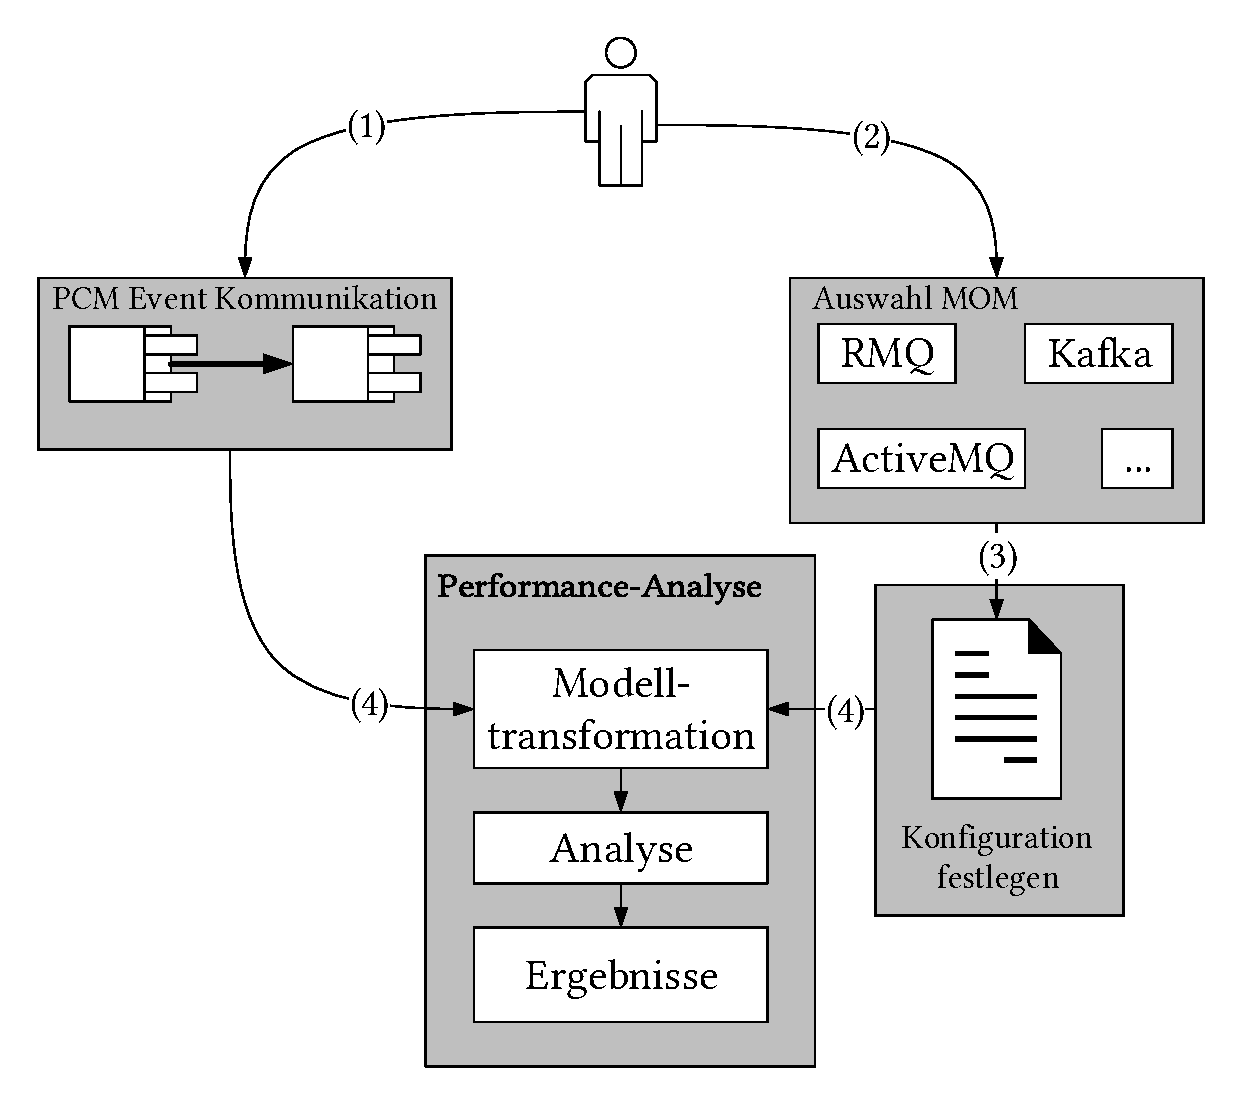
\includegraphics[width=1\textwidth]{images/transformation/transformationOverview.pdf}
  \caption{Übersicht des Transformationsprozess}
  \label{img:transformationOverview}
\end{figure}


\section{Konfiguration der MOM}
Wie bereits in den vorherigen Kapitel beschrieben, haben verschiedene MOMs auch diverse Möglichkeiten konfiguriert zu werden. Damit ein Architekt auch Konfigurationen einer MOM untersuchen kann, soll ihm die Möglichkeit geboten werden, bestimmte Konfigurationen einer MOM angeben zu können. Die möglichen Konfigurationen sind von der jeweiligen MOM abhängig. Für RMQ, die in dieser Masterarbeit untersuchte MOM, könnten folgende Konfigurationen angeboten werden:
\begin{itemize}
    \item Bereitstellen von Warteschlange: Welche Warteschlange wird auf welcher Ressource bereitgestellt. Dabei wird der Name des \emph{EventType}s angegeben, welchen die Warteschlange verarbeiten soll. Die Ressource auf der die Warteschlange bereitgestellt werden soll muss vor der Transformation bereits existieren. Außerdem kann Durchsatz und Latenz zu dieser Warteschlange angegeben werden.
    \item Lazy-Warteschlangen: Dabei kann angegeben werden ob die bereitgestellte Warteschlange eine Lazy-Warteschlange ist oder nicht. 
    \item Exchange-Zuständigkeit: Dabei kann festgelegt werden welche Warteschlange an welchen Exchange gebunden wird. Dabei kann ein Name für den Exchange und die Namen der dazugehörigen Warteschlangen angegeben werden. Der Name der Warteschlange ist dabei der \emph{EventType}, welchen die Warteschlange verarbeitet.
    \item Bereitstellen eines Exchange: Auf welcher Ressource wird der Exchange bereitgestellt. Außerdem kann Durchsatz und Latenz zu diesem Exchange angegeben werden.
\end{itemize}
In \autoref{img:configExample} ist eine Möglichkeit abgebildet, wie ein Architekt eine Konfiguration für einen RMQ-Baustein angeben kann. Dabei handelt es sich um eine XML-Datei. Zu sehen ist, dass es zwei Warteschlangen gibt. Die erste verarbeitet Nachrichten vom \emph{EventType} \texttt{Order}. Sie ist wird auf der Ressource \texttt{Middleware} bereitgestellt und ist eine Lazy-Warteschlange. Die zweite Warteschlange verarbeitet Nachrichten vom \emph{EventType} \texttt{OrderConf}. Auch sie wird auf der Ressource \texttt{Middleware} bereitgestellt. Sie ist jedoch keine Lazy-Warteschlange. Beide Warteschlange haben keinen Durchsatz und Latenz angegeben. Außerdem gibt es nur einen Exchange. Dieser wird ebenfalls auf der \texttt{Middleware} Ressource bereitgestellt. Er hat einen Durchsatz in Bytes und eine Latenz in Millisekunden angegeben. Die von ihm verwalteten Warteschlangen sind die beiden zuvor definierten Warteschlangen. Die hier vorgestellte Konfigurationsdatei ist nur ein Vorschlag, wie eine mögliche Konfiguration aussehen kann. Die Konfiguration kann auch in anderen Formen in die Transformation eingebunden werden, z.B. mithilfe von PCM-Profiles \cite{kramer2012b}.



\begin{figure}
\center
  \lstinputlisting[language=XML]{code/configExample.xml}
  \caption{Beispiel einer möglichen XML-Konfiguration für einen RMQ-Baustein.}
  \label{img:configExample}
\end{figure}

\section{Generierung von Exchange und Warteschlangen}
In \autoref{img:transformationRepository} ist die Transformation des Repository-Modells abgebildet. Im Ersten Schritt werden im Repository-Modell \emph{Exchange}-Komponenten eingefügt. Dabei wird die Anzahl und die Namen aus der Konfigurationsdatei ausgelesen. Außerdem werden die Ressourcen Anforderungen für Latenz und Durchsatz an die passende Stelle, der jeweiligen \texttt{Exchange}-Komponente, eingesetzt. Diese wurden in \autoref{sec:rmqRd} beschrieben. Die Komponenten werden wie im vorherigen Kapitel angeboten. Im nächsten Schritt wird jeder Sender identifiziert, der ein \emph{EventType} aussendet. Für diese Sender werden jeweils eine \emph{requiredRole} eingefügt, die eine der zuvor eingefügten \texttt{Exchange}-Komponente benötigt. Dabei werden die \emph{EventType}s beachtet. Jede \emph{EmitEventAction} eines Senders wird nun durch eine \emph{ExternalCallAction} ersetzt, die in der jeweiligen \texttt{Exchange}-Komponente die Funktion \texttt{Exchange.distribute} aufruft. Mithilfe einer \emph{UsageVariable} wird die Parameterbelegung festgelegt. Dabei wird als Typ der Name der zuvor aussendenden \emph{EventAction} angegeben. Außerdem wird eine Warteschlangen-Komponente angelegt die Nachrichten vom Typ \emph{EventType.name} entgegen nimmt. Bei der Erstellung werden außerdem passende Ressourcenanforderungen für eine Nachricht eingefügt. Diese werden aus der MOM-Konfiguration entnommen und an den passenden Stellen eingesetzt. Dies wurde in \autoref{sec:rmqRd} beschrieben. In der jeweiligen \texttt{Exchange}-Komponente, der für diesen \emph{EventType} zuständig ist, wird eine \emph{requiredRole} eingefügt, die diese Warteschlange benötigt. Als nächstes wird in den \texttt{distribute}-SEFF der \texttt{Exchange}-Komponente ein \emph{GuardedBranch} eingefügt. Die Bedingung lautet \texttt{Type == EventType.name}. Im Anschluss wird eine \emph{ExternalCallAction} eingefügt die die \texttt{Queue.put} Funktion in der zuvor erstellten Warteschlangen-Komponente aufruft. Nachdem alle Sender abgearbeitet wurden, wird nach allen Empfängern gesucht, die einen \emph{EventType} handhaben. Zunächst wird für diesen \emph{EventType} eine Schnittstelle mit dem Namen \texttt{IRecvX}, mit \texttt{X = EventType.name} angelegt. Diese Schnittstelle hat eine Signatur mit dem Namen \texttt{recvX}. Die Schnittstelle wird von dem aktuell betrachteten Empfänger angeboten. Außerdem wird eine \emph{requiredRole} erstellt, die die \texttt{Exchange}-Komponente benötigt, die dem \emph{EventType} zugeordnet ist. Ein SEFF wird erstellt, der die Funktionalität von \texttt{IRecvX.recvX} abbilden soll. Dieser enthält einen \emph{ExternalCallAction}, die die \texttt{Exchange.receive} in der benötigten \texttt{Exchange}-Komponente aufruft. Die Parameterbelegung wird mit einer \emph{UsageVariable}, mit \texttt{Type = EventType.name}, angegeben. Als nächstes wird im \texttt{receive}-SEFF der \texttt{Exchange}-Komponente eine \emph{BranchAction} eingefügt. Die Bedingung lautet \texttt{Type == EventType.name}. Im Anschluss wird eine \emph{ExternalCallAction} eingefügt die die \texttt{Queue.get} Funktion in der Warteschlangen Komponente aufruft, die Nachrichten vom Typ \emph{EventType} beinhalten.

\begin{figure}
\center
  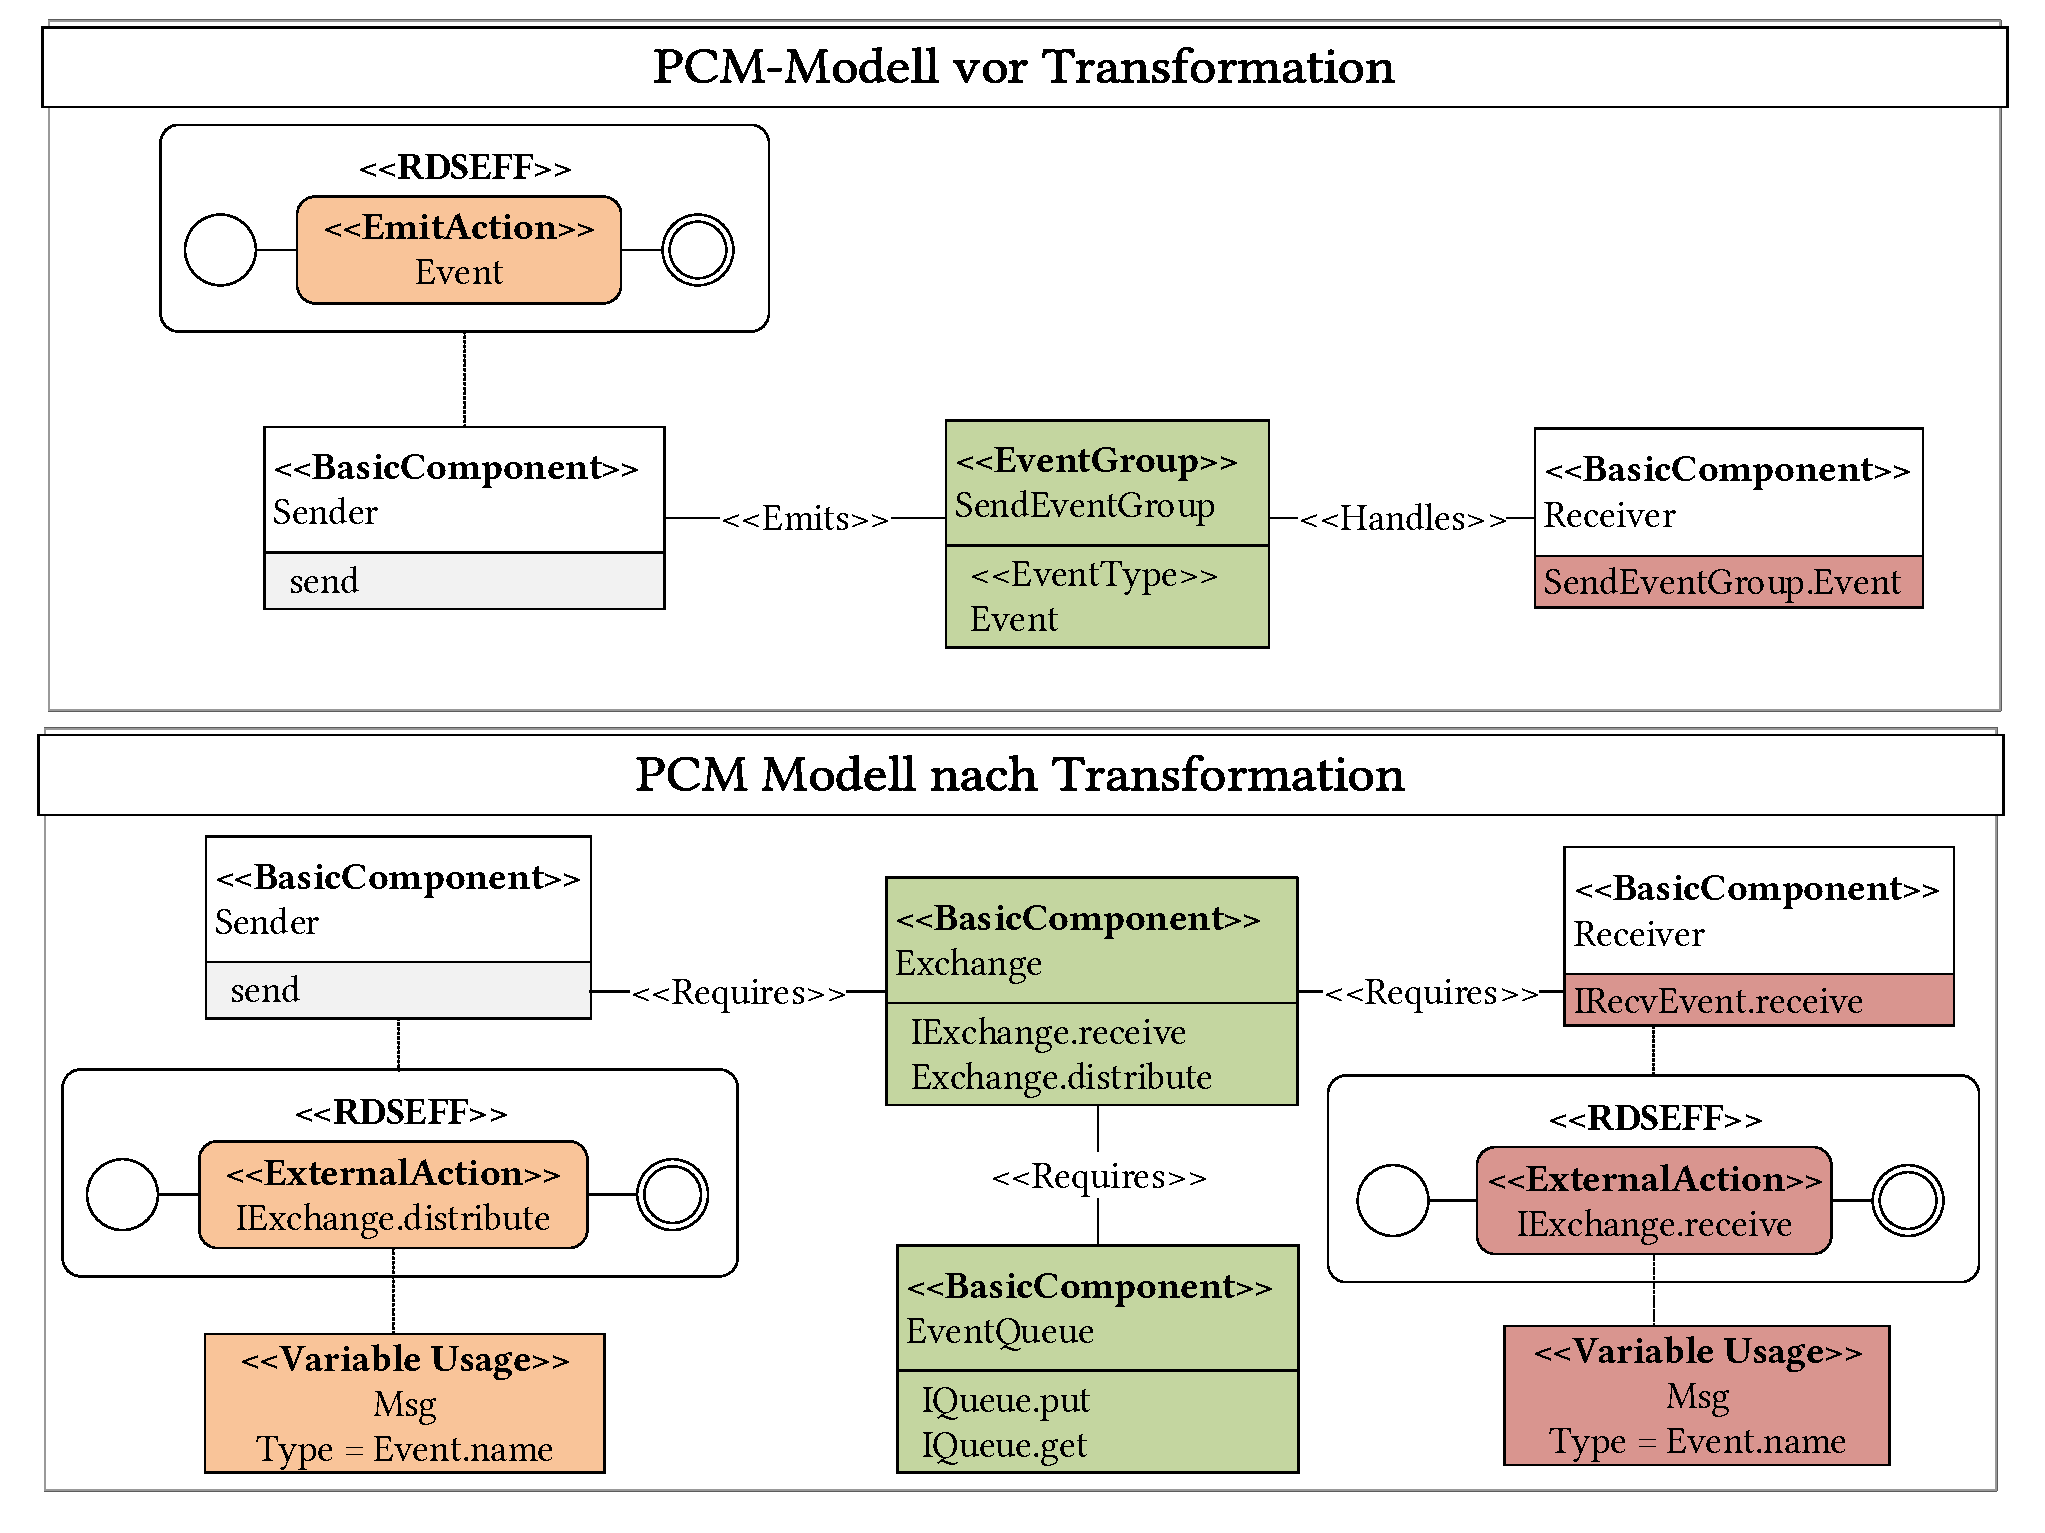
\includegraphics[width=1.3\textwidth, angle=90]{images/transformation/transformationRepository.pdf}
  \caption{Übersicht der Repository-Modell-Transformation}
  \label{img:transformationRepository}
\end{figure}


\section{Transformation von Punkt-Zu-Punkt Kommunikation}
Im Folgenden wird beschrieben, wie die Punkt-Zu-Punkt Kommunikation zwischen Komponenten transformiert wird. Eine Übersicht ist in \autoref{img:transformationP2P} abgebildet. Dabei wird das System- und Nutzungsmodell transformiert. Als erster Schritt werden die zuvor erstellen Exchange- und Warteschlangen-Komponenten im Systemmodell in einem \emph{AssemblyContext} eingefügt. Im Anschluss werden alle Warteschlangen mit der jeweiligen Exchange-Komponente über die passende Schnittstelle mit einem \emph{AssemblyConnector} verbunden. Als nächstes werden alle \emph{AssemblyEventConnector}s gesucht. Jeder \emph{AssemblyEventConnector} hat ein \emph{SourceRole} und ein \emph{SinkRole} Feld. Für jede \emph{SourceRole} wird die darin enthaltene Komponente über einen \emph{AssemblyConnector} mit der Exchange-Komponente verbunden. Die Komponente die sich im \emph{SinkRole}-Feld befindet wird ebenfalls mit der Exchange-Komponente, mithilfe eines \emph{AssemblyConnector}, verbunden. Außerdem wird für jedes der \emph{SinkRole}-Elemente eine \emph{SystemProvidedRole} erstellt. Die \emph{SinkRole}-Komponente und die \emph{SystemProvidedRole} werden mit einem \emph{DelegationsConnector} verbunden. Schließlich wird im Nutzungsmodell ein \emph{UsageScenario} angelegt um das Abholen von Nachrichten abzubilden. Dazu wird in dem \emph{UsageScenario} ein \emph{EntryLevelSystemCall} angelegt, der über die jeweilige \emph{SystemProvidedRole} Funktion \texttt{Exchange.receive} aufruft. Außerdem wird ein \emph{ClosedWorkload} mit \emph{Population} eins und einer \emph{ThinkTime} von null angelegt. Dadurch wird gewährleistet, dass eine Empfänger-Komponenten eine Nachricht aus der Warteschlange holt, sobald diese Verfügbar ist.

\begin{figure}
\center
  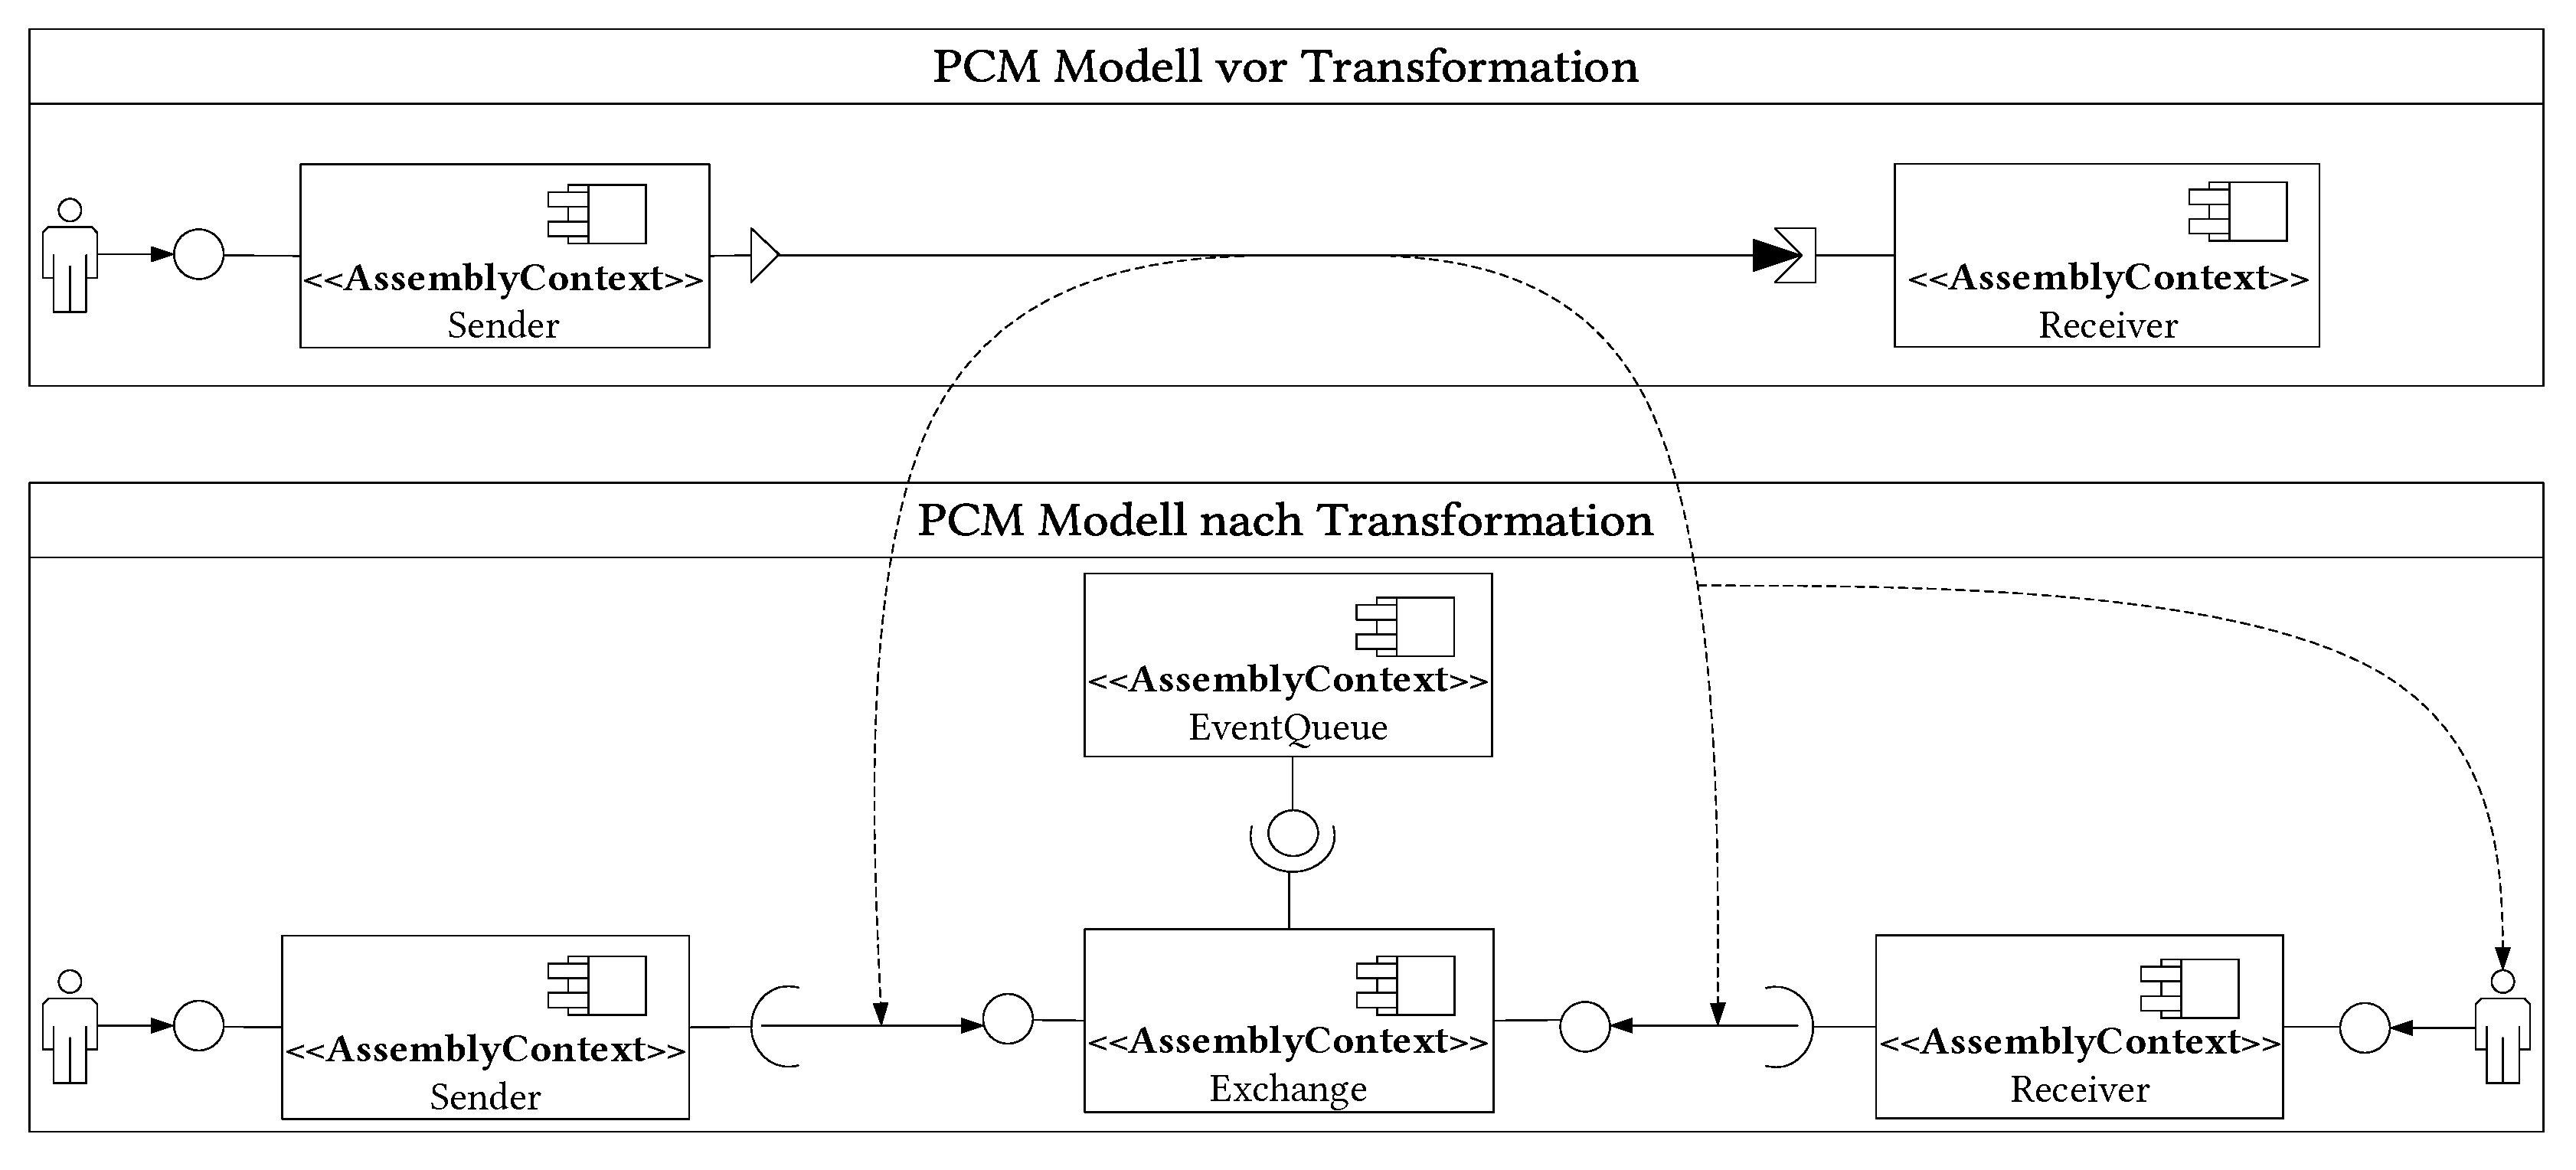
\includegraphics[width=1.3\textwidth, angle=90]{images/transformation/transformationSystemP2P.pdf}
  \caption{Übersicht der Punkt-Zu-Punkt-Transformation}
  \label{img:transformationP2P}
\end{figure}

\section{Transformation von Viele-Zu-Viele Kommunikation}
Im Fall von Viele-Zu-Viele Kommunikation werden neben dem System- und Nutzungsmodell auch das Repository-Modell angepasst. Eine Übersicht ist in \autoref{img:transformationPubSub} abgebildet. Die Viele-Zu-Viele Kommunikation findet in PCM über einen \emph{EventChannel} statt. Sender sind über eine \emph{SourceConnector} und Empfänger über einen \emph{SinkConnector} mit dem \emph{EventChannel} verbunden. Für jeden \emph{SourceConnector}, der die Sender-Komponente mit dem \emph{EventChannel} verbindet, wird ein \emph{AssemblyConnector} zwischen dem Sender und der jeweiligen Exchange-Komponente erstellt. Bei der Transformation der \emph{SinkConnector}en wird zunächst ein neuer \emph{AssemblyContext} mit Warteschlangen-Komponente erstellt. Im Repository-Modell wird in der Exchange-Komponente eine neue \emph{RequiredRole} angelegt die diese Warteschlange benötigt. Im \texttt{distribute}-SEFF wird der \emph{GuardedBranch} erweitert, der den dazugehörige \emph{EventType} behandelt. Für die zuvor erstellte \emph{RequiredRole} wird eine weiterer \emph{ExternalCallAction} erstellt, der die Nachricht an die Warteschlange sendet. Somit wird die Nachricht an mehrere Warteschlangen weitergeleitet. Im Systemmodell wird mit einem \emph{AssemblyConnector} die Exchange-Komponente und die Warteschlange verbunden. Außerdem wird für den Empfänger-\emph{AssemblyContext} eine \emph{SystemProvidedRole} erstellt und mit dem \emph{AssemblyContext}, mithilfe eines \emph{DelegationsConnector}s, verbunden. Schließlich wird, wie auch bei der Punkt-Zu-Punkt Transformation, im Nutzungsmodell eine \emph{UsageScanrio} angelegt. Damit soll das Abholen von Nachrichten abgebildet werden. In dem \emph{UsageScenario} wird ein \emph{EntryLevelSystemCall} angelegt, der über die jeweilige \emph{SystemProvidedRole} die \texttt{Exchange.receive} Funktion aufruft. Außerdem wird ein \emph{ClosedWorkload} mit \emph{Population} eins und einer \emph{ThinkTime} von null angelegt, damit eine Nachricht aus der Warteschlange geholt wird, sobald diese Verfügbar ist.

\begin{figure}
\center
  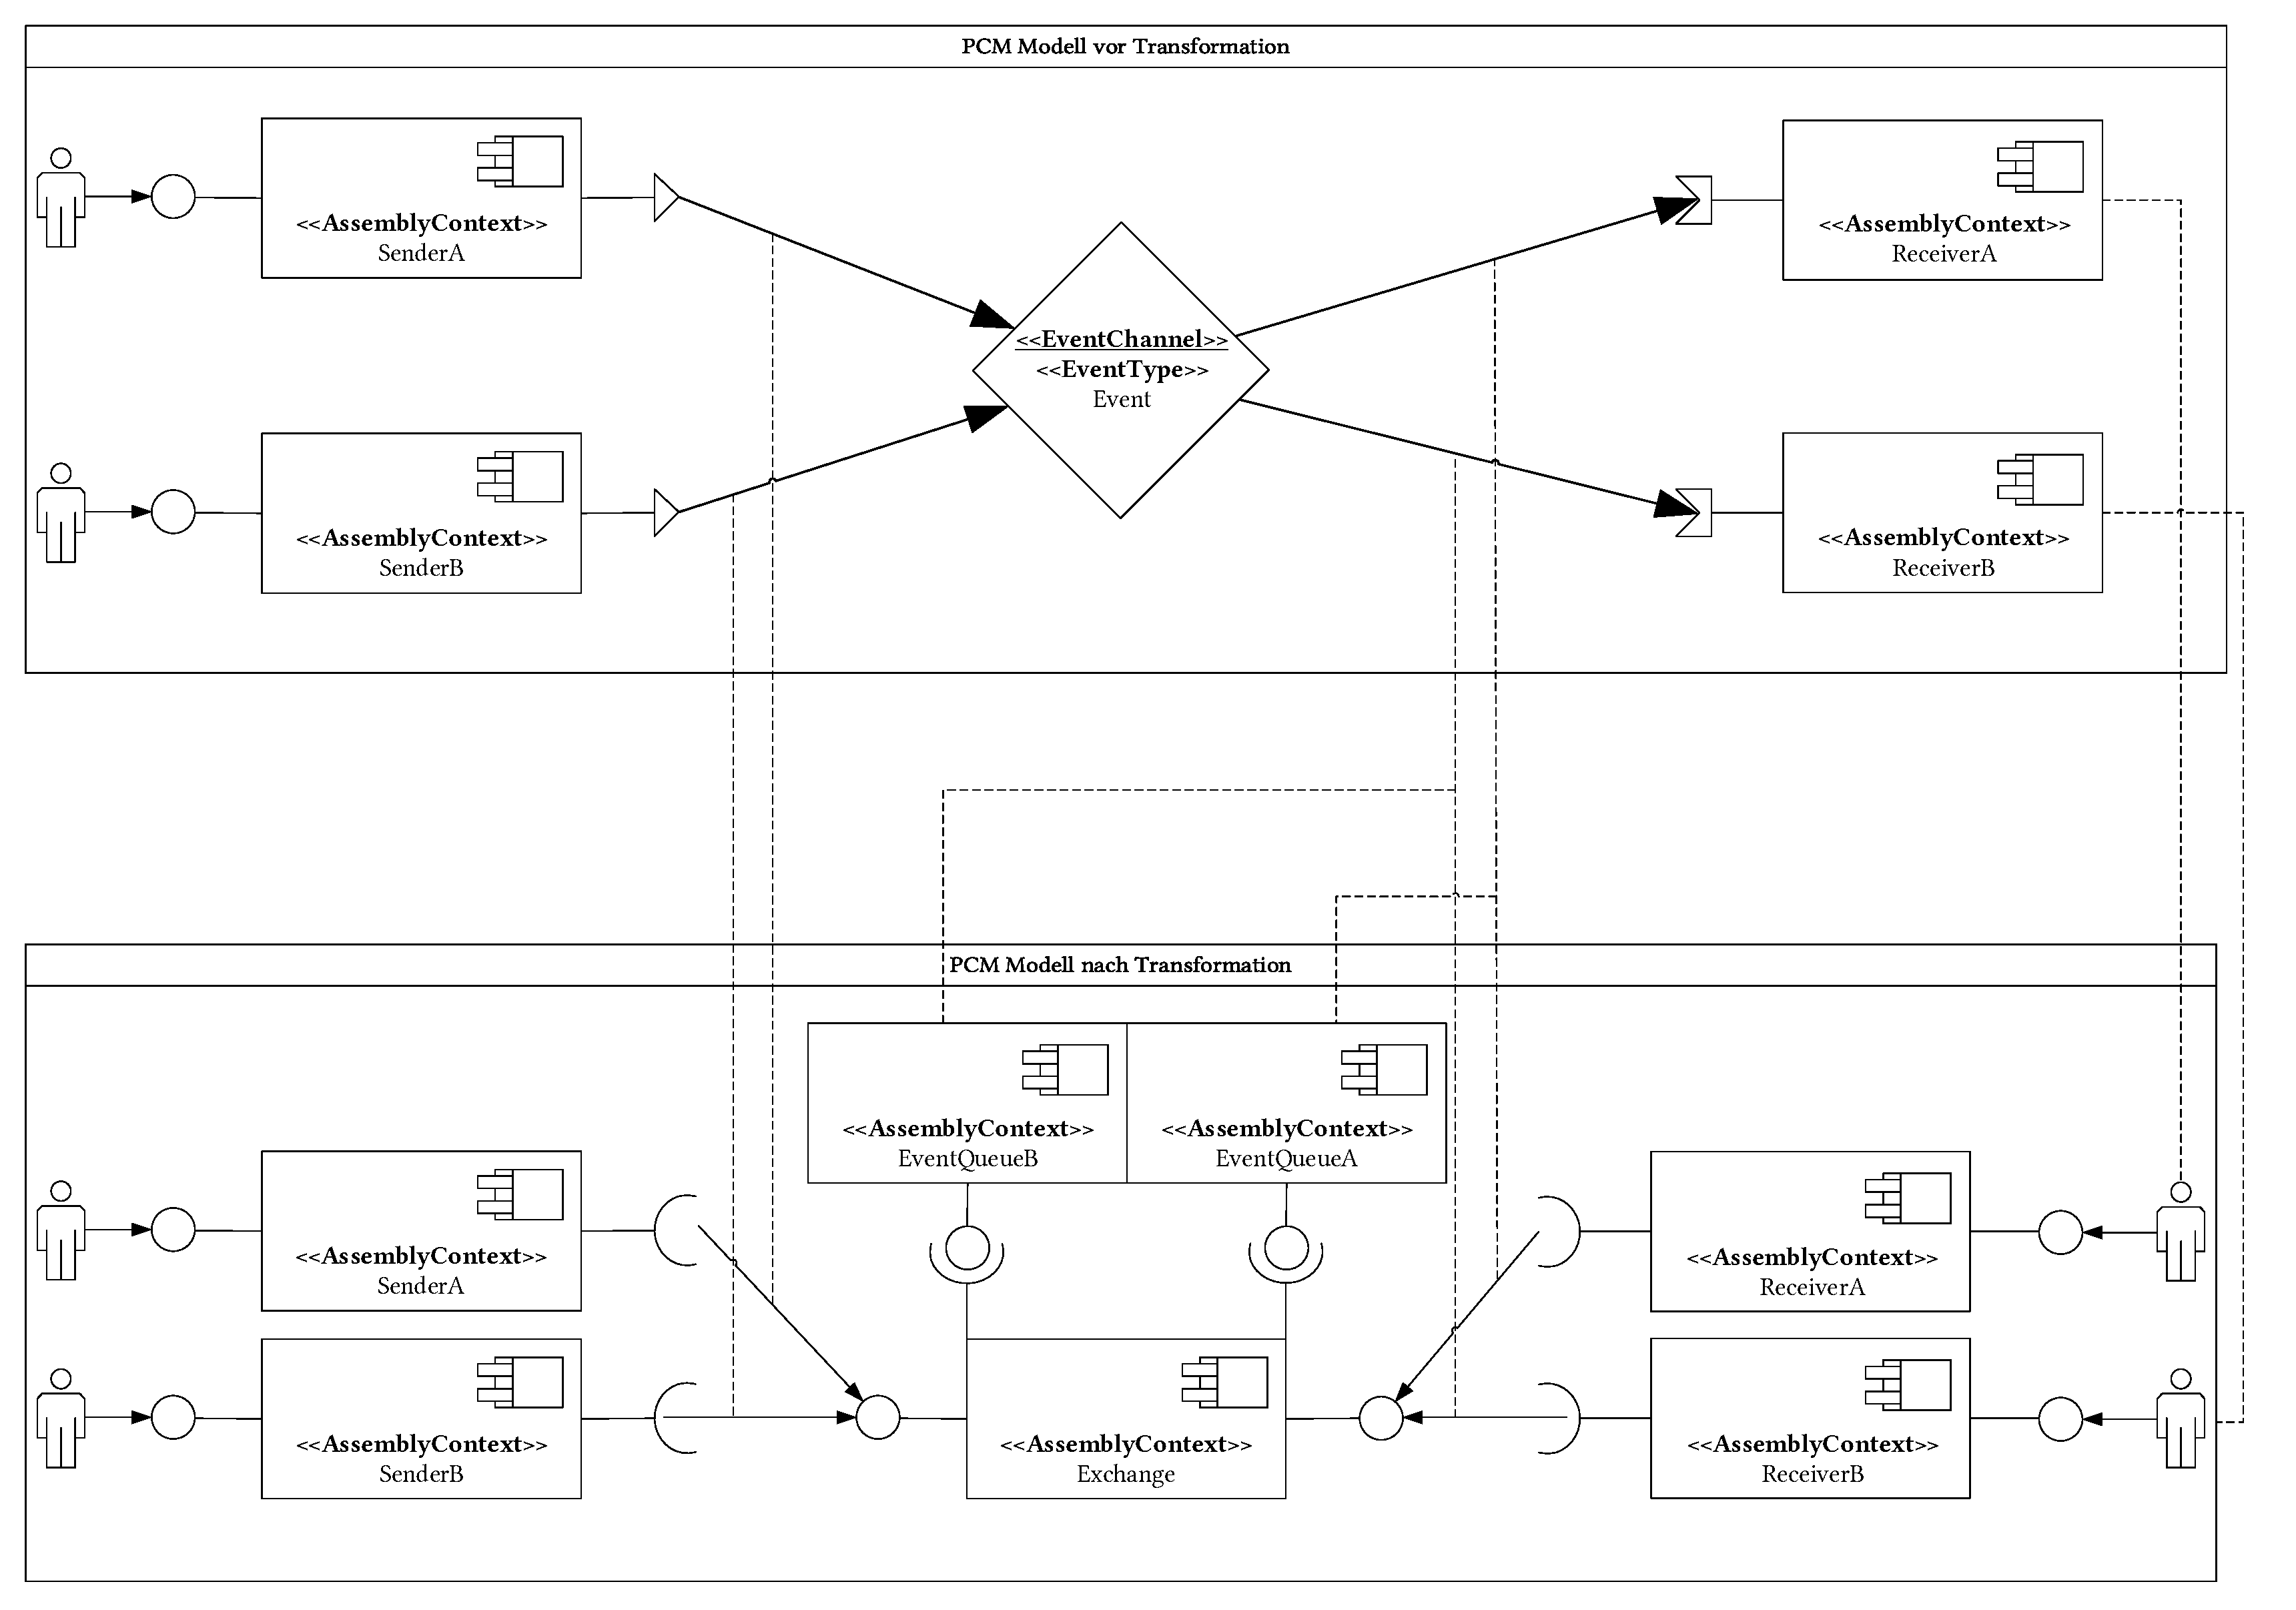
\includegraphics[width=1.4\textwidth, angle=90]{images/transformation/transformationSystemPubSub.pdf}
  \caption{Übersicht der Publish/Subscribe-Transformation}
  \label{img:transformationPubSub}
\end{figure}


\section{Bereitstellen der Komponenten}
Das Bereitstellen der Komponenten setzt voraus, dass in der vom Benutzer angegebenen Konfiguration festgelegt wurde, welche Warteschlangen- und Exchange-Komponente auf welcher Ressource bereitgestellt werden soll. Diese Ressourcen müssen bereits vor der Transformation erstellt worden sein. Währende der Transformation werden die Komponenten auf den Ressourcen im Allokations-Modell bereitgestellt. Dazu wird ein \emph{AllocationContext} erstellt auf der dazugehörigen Ressource bereitgestellt.

